\documentclass[11pt]{article}

\usepackage{latexsym}
\usepackage{amsmath}
\usepackage{amssymb}
\usepackage{amsthm}
\usepackage{graphicx}
\usepackage{wrapfig}
\usepackage{pseudocode}
\usepackage{url}
\usepackage[backref, colorlinks=true, citecolor=red, urlcolor=blue, pdfauthor={Jyh-Ming Lien}]{hyperref}


\newcommand{\handout}[5]{
  \noindent
  \begin{center}
  \framebox{
    \vbox{
      \hbox to 5.78in { {\bf } \hfill #2 }
      \vspace{4mm}
      \hbox to 5.78in { {\Large \hfill #5  \hfill} }
      \vspace{2mm}
      \hbox to 5.78in { {\em #3 \hfill #4} }
    }
  }
  \end{center}
  \vspace*{4mm}
}

\newcommand{\lecture}[4]{\handout{#1}{#2}{#3}{}{Report for #3}}

\newtheorem{theorem}{Theorem}
\newtheorem{corollary}[theorem]{Corollary}
\newtheorem{lemma}[theorem]{Lemma}
\newtheorem{observation}[theorem]{Observation}
\newtheorem{proposition}[theorem]{Proposition}
\newtheorem{definition}[theorem]{Definition}
\newtheorem{claim}[theorem]{Claim}
\newtheorem{fact}[theorem]{Fact}
\newtheorem{assumption}[theorem]{Assumption}

% 1-inch margins, from fullpage.sty by H.Partl, Version 2, Dec. 15, 1988.
\topmargin 0pt
\advance \topmargin by -\headheight
\advance \topmargin by -\headsep
\textheight 8.9in
\oddsidemargin 0pt
\evensidemargin \oddsidemargin
\marginparwidth 0.5in
\textwidth 6.5in

\parindent 0in
\parskip 1.5ex
%\renewcommand{\baselinestretch}{1.25}

\begin{document}
 
\lecture{Advance Algorithm Programming Assignment 1 }{Fall 2015}{Yunjoo Park}{---}


\section{Implementation Details}
\subsection{Problem-solving methods and algorithms}
The \textit{crust algorithm} is a algorithm for the reconstruction of surfaces of arbitary topolgy from unorganized sample points in 3D\cite{crust-algorithm}. The input to the algorithm is a set $S$ of sample points from the surface of a three-dimensional object\cite{crust-algorithm-nina}. Let  $P := \{p_1,p_2,...,p_n\}$ be a set of 3D points in the plane. For the crust, firstly, we have to compute the \textit{Voronoi diagram} $V_p$ of the sample points $P$. A Voronoi diagram is a partitioning of plae into regions based on distance to points in a specific subset of the plane. The Voronoi diagram is dual to its \textit{Delaunay triangulation}. For each sample point $p$, find the two vertices of $V_p$ fathest from $p$. One is a pole and the other is antipole of $s$. And then, union the sample points and poles. For the union, compute the \textit{Delaunay Triangulation}. From the triangulation, discard some triangle with a pole as a vertex and keep only triangles for which all three vertices are sample points in $P$.

\subsection{Platforms}
Languages: C

Platform: Microsoft visual Studio 2013

\subsection{Examples of Inputs}
\begin{figure}[hbt]
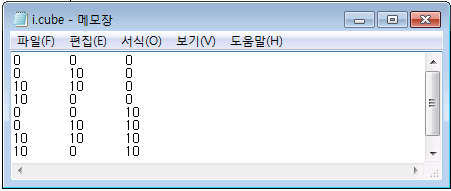
\includegraphics[width=.5\textwidth]{FIGS/inputs}
\centering
\caption{An Example of inputs}
\end{figure}
1. There are 12 test data.

2. Each data file has different values.

3. Each line is a 3D point ($x, y, z$).

\subsection{Problem-solving methods and algorithms}
For lifting the given points to 4D, add another point $pt4 = x^2+y^2+z^2$. For new set of points, I compute a voronoi diagram by using qhull\cite{qhull-library} and get a voronoi vertices of facet lowerdelaunay. Then, find a pole and antipole for all points. If a point $o$ lies on the convex hull, the pole vector $\vec{po}$ is the average of the outer nomals of the adjacents. On the other hand, if a point does not lie on the convex hull, the pole is the farthest voronoi vertex of voronoi vertices from the point. And then, compute the other pole, antipole. An antipole is a vertex farthes away from the point $o$ in direction of $\vec{op}$. By using inner product, find the antipole. And then, add poles and antipoles into $vertices$. For the new set $vertices$, compute the Delaunay Triangulation. The poles have a member variable, $ispole$. By using this value, report triangles whose vertices are all from original set $P$.

\section{Example Output}
\begin{figure}[ht]
\centering
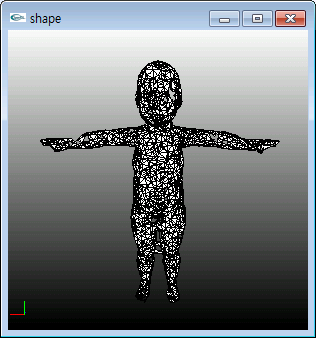
\includegraphics[width=.23\textwidth]{FIGS/bb1}
\hspace{0.2cm}
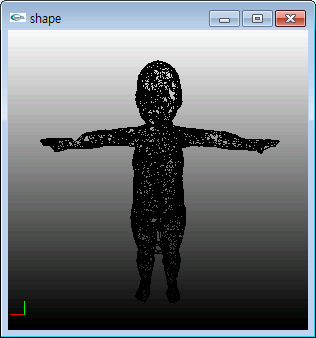
\includegraphics[width=.23\textwidth]{FIGS/bb2}
\hspace{0.2cm}
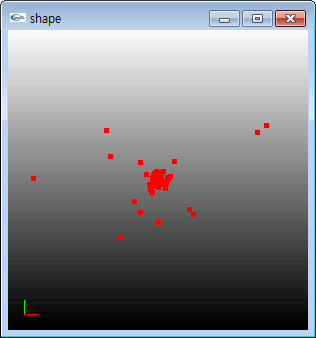
\includegraphics[width=.23\textwidth]{FIGS/bb3}
\hspace{0.2cm}
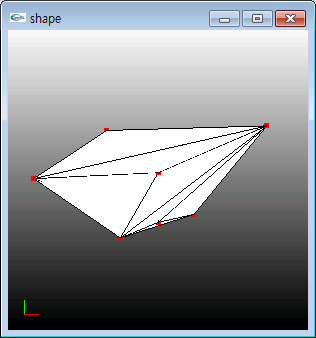
\includegraphics[width=.23\textwidth]{FIGS/bb4}
\caption{i.bb}
\end{figure}
\begin{figure}[ht]
\centering
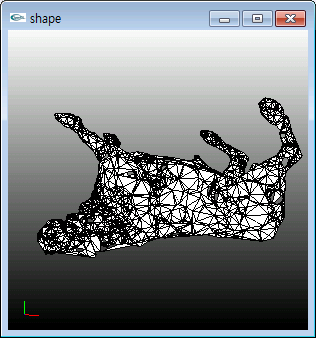
\includegraphics[width=.23\textwidth]{FIGS/bull1}
\hspace{0.2cm}
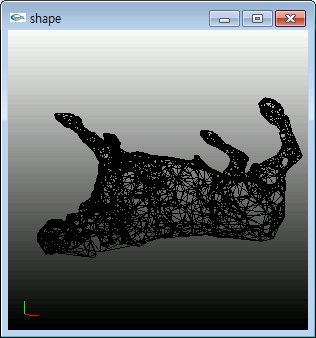
\includegraphics[width=.23\textwidth]{FIGS/bull2}
\hspace{0.2cm}
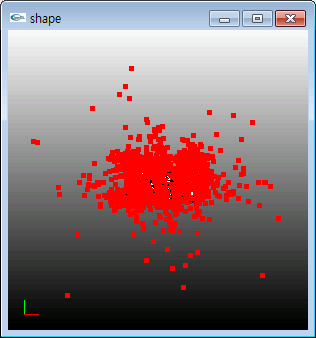
\includegraphics[width=.23\textwidth]{FIGS/bull3}
\hspace{0.2cm}
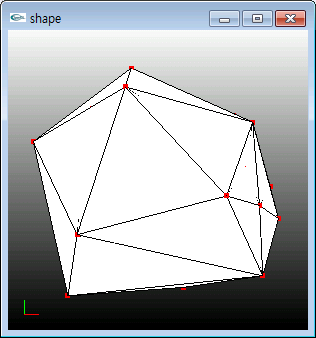
\includegraphics[width=.23\textwidth]{FIGS/bull4}
\caption{i.bull}
\end{figure}

\begin{figure}[ht]
\centering
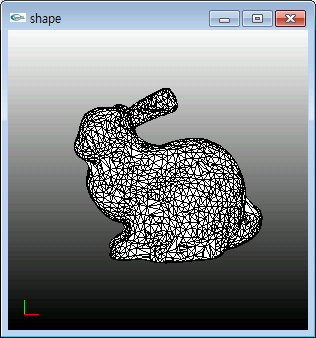
\includegraphics[width=.23\textwidth]{FIGS/bunny1}
\hspace{0.2cm}
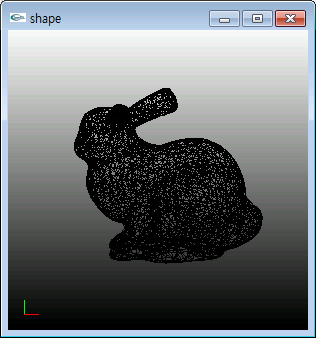
\includegraphics[width=.23\textwidth]{FIGS/bunny2}
\hspace{0.2cm}
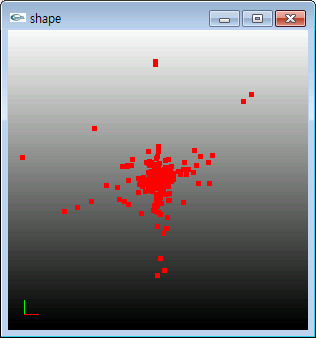
\includegraphics[width=.23\textwidth]{FIGS/bunny3}
\hspace{0.2cm}
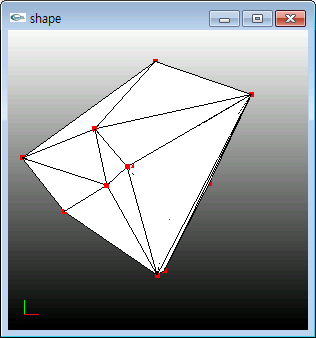
\includegraphics[width=.23\textwidth]{FIGS/bunny4}
\caption{i.bunny}
\end{figure}

\begin{figure}[ht]
\centering

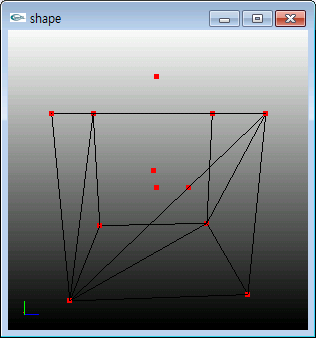
\includegraphics[width=.23\textwidth]{FIGS/cube2}
\hspace{0.2cm}
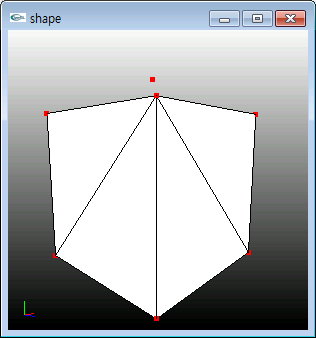
\includegraphics[width=.23\textwidth]{FIGS/cube3}
\hspace{0.2cm}
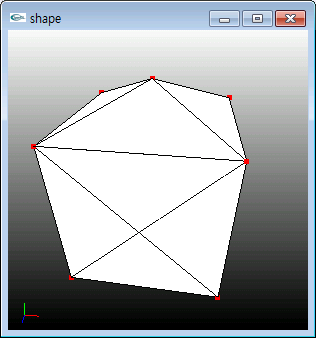
\includegraphics[width=.23\textwidth]{FIGS/cube4}
\caption{i.cube}
\end{figure}

\begin{figure}[ht]
\centering
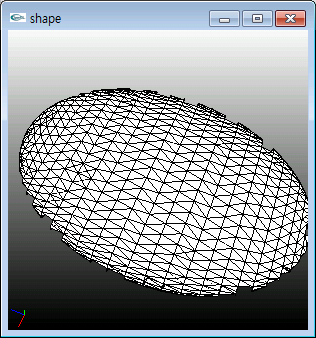
\includegraphics[width=.23\textwidth]{FIGS/ellipsoid1}
\hspace{0.2cm}
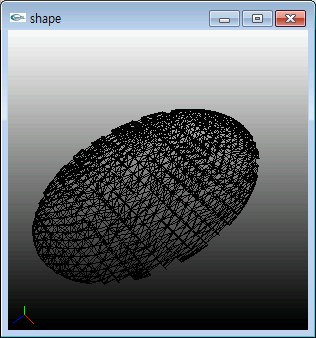
\includegraphics[width=.23\textwidth]{FIGS/ellipsoid2}
\hspace{0.2cm}
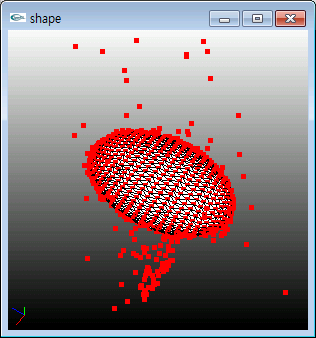
\includegraphics[width=.23\textwidth]{FIGS/ellipsoid3}
\hspace{0.2cm}
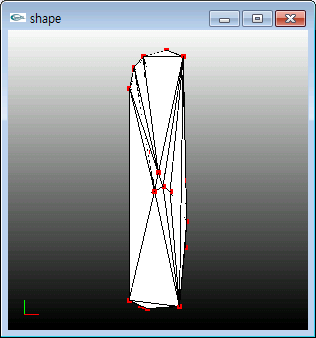
\includegraphics[width=.23\textwidth]{FIGS/ellipsoid4}
\caption{i.ellipsoid}
\end{figure}

\begin{figure}[ht]
\centering
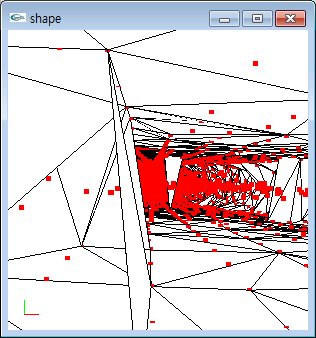
\includegraphics[width=.23\textwidth]{FIGS/screwdriver}
\hspace{0.5cm}
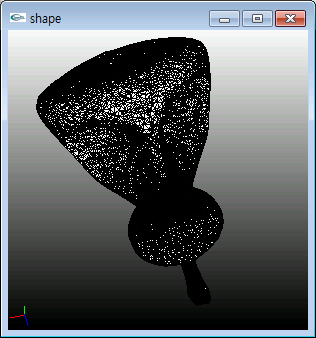
\includegraphics[width=.23\textwidth]{FIGS/screwdriver1}
\hspace{0.5cm}
\vspace{0.5cm}
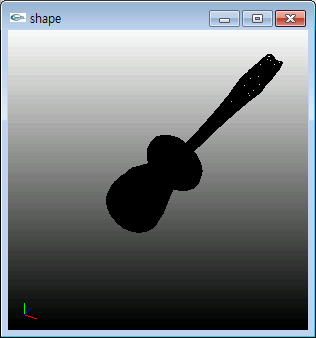
\includegraphics[width=.23\textwidth]{FIGS/screwdriver2}
\hspace{0.5cm}
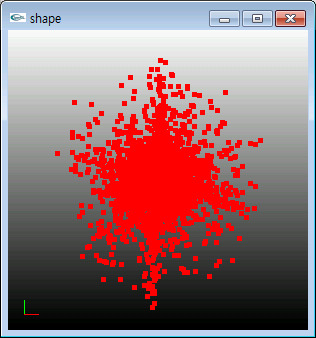
\includegraphics[width=.23\textwidth]{FIGS/screwdriver3}
\hspace{0.5cm}
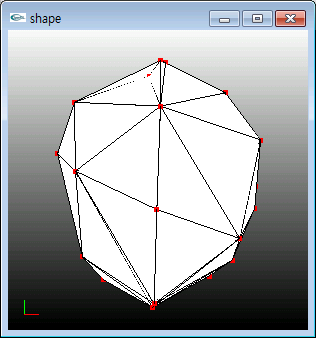
\includegraphics[width=.23\textwidth]{FIGS/screwdriver4}
\caption{i.screwdriver}
\end{figure}

\begin{figure}[ht]
\centering
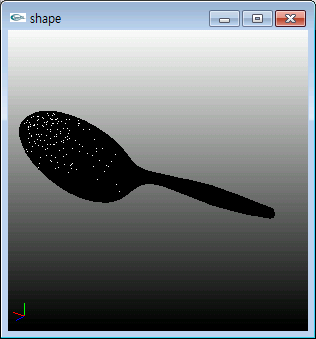
\includegraphics[width=.23\textwidth]{FIGS/spoon1}
\hspace{0.2cm}
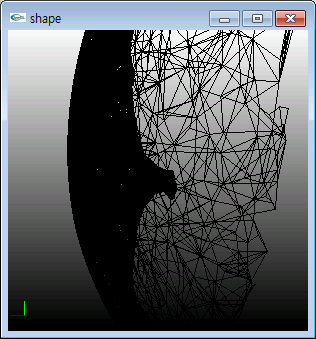
\includegraphics[width=.23\textwidth]{FIGS/spoon2}
\hspace{0.2cm}
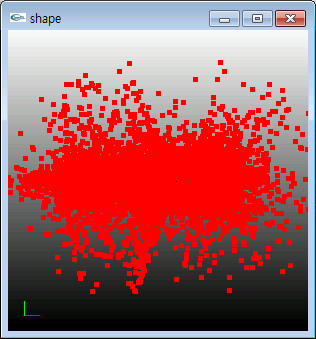
\includegraphics[width=.23\textwidth]{FIGS/spoon3}
\hspace{0.2cm}
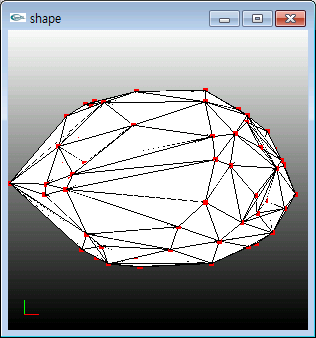
\includegraphics[width=.23\textwidth]{FIGS/spoon4}
\caption{i.spoon}
\end{figure}

\begin{figure}[ht]
\centering
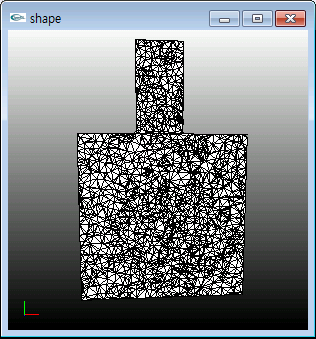
\includegraphics[width=.23\textwidth]{FIGS/T1}
\hspace{0.2cm}
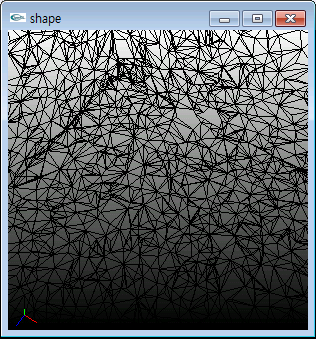
\includegraphics[width=.23\textwidth]{FIGS/T2}
\hspace{0.2cm}
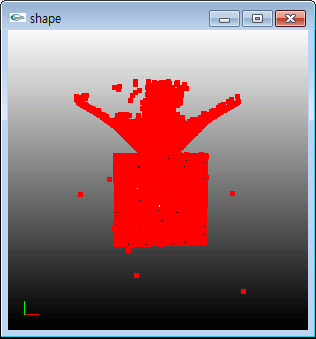
\includegraphics[width=.23\textwidth]{FIGS/T3}
\hspace{0.2cm}
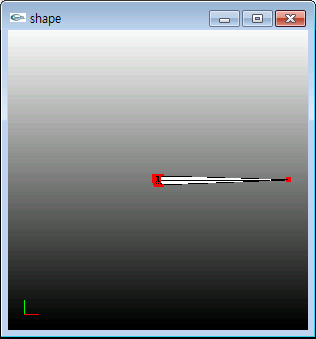
\includegraphics[width=.23\textwidth]{FIGS/T4}
\caption{i.T}
\end{figure}

\begin{figure}[ht]
\centering
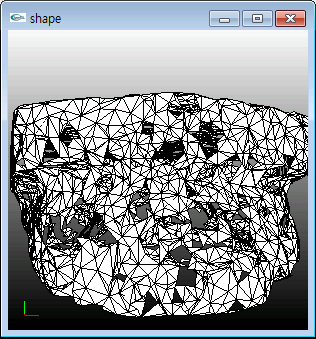
\includegraphics[width=.23\textwidth]{FIGS/teeth1}
\hspace{0.2cm}
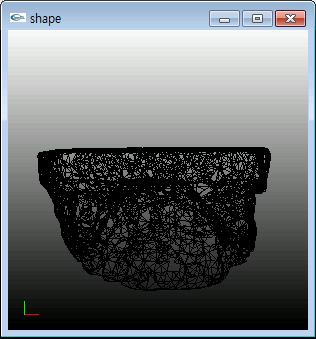
\includegraphics[width=.23\textwidth]{FIGS/teeth2}
\hspace{0.2cm}
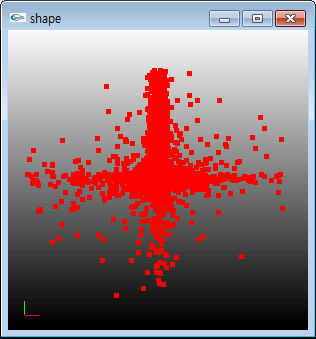
\includegraphics[width=.23\textwidth]{FIGS/teeth3}
\hspace{0.2cm}
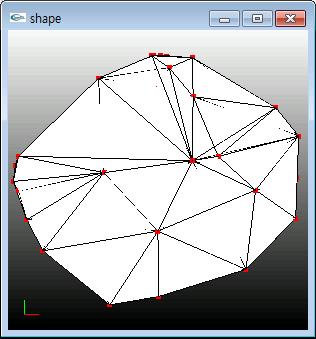
\includegraphics[width=.23\textwidth]{FIGS/teeth4}
\caption{i.teeth}
\end{figure}

\begin{figure}[ht]
\centering
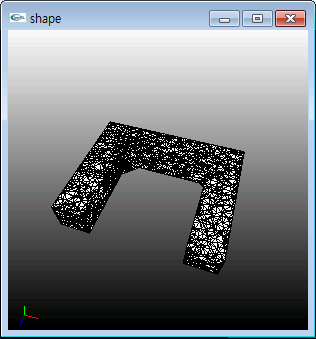
\includegraphics[width=.23\textwidth]{FIGS/U1}
\hspace{0.2cm}
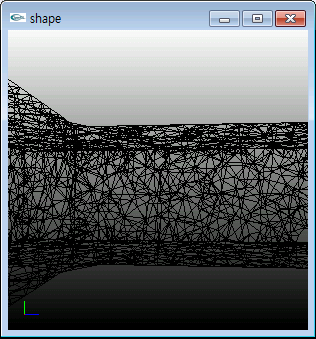
\includegraphics[width=.23\textwidth]{FIGS/U2}
\hspace{0.2cm}
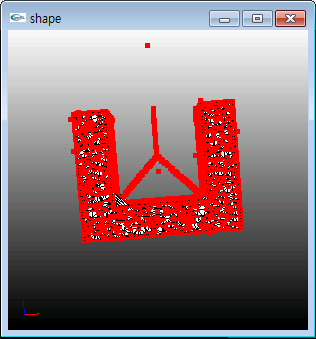
\includegraphics[width=.23\textwidth]{FIGS/U3}
\hspace{0.2cm}
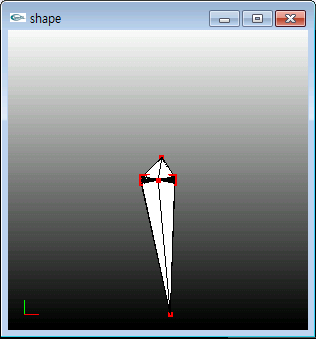
\includegraphics[width=.23\textwidth]{FIGS/U4}
\caption{i.U}
\end{figure}

\begin{figure}[ht]
\centering
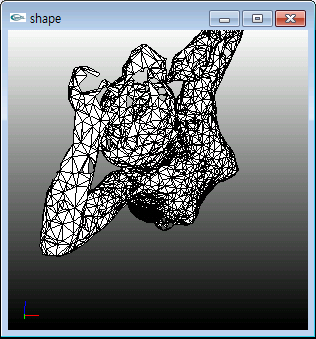
\includegraphics[width=.23\textwidth]{FIGS/woman1}
\hspace{0.2cm}
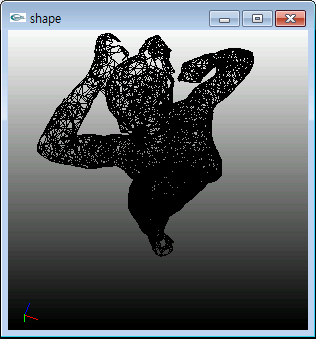
\includegraphics[width=.23\textwidth]{FIGS/woman2}
\hspace{0.2cm}
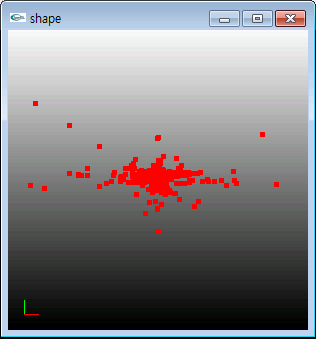
\includegraphics[width=.23\textwidth]{FIGS/woman3}
\hspace{0.2cm}
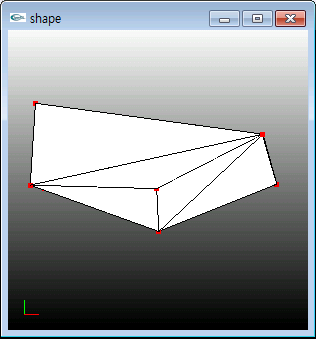
\includegraphics[width=.23\textwidth]{FIGS/woman4}
\caption{i.woman}
\end{figure}

\begin{figure}[ht]
\centering
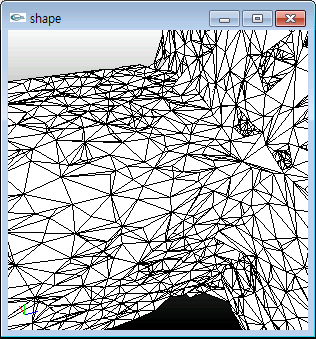
\includegraphics[width=.23\textwidth]{FIGS/Y1}
\hspace{0.2cm}
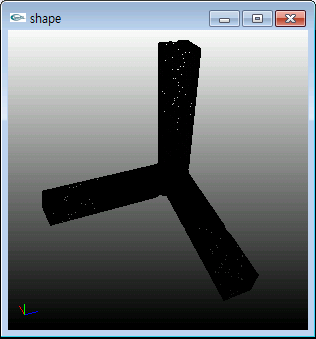
\includegraphics[width=.23\textwidth]{FIGS/Y2}
\hspace{0.2cm}
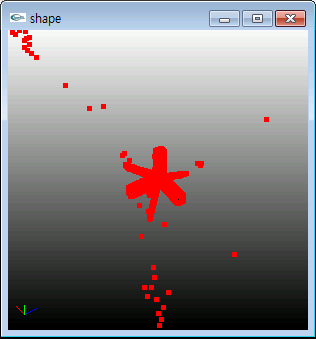
\includegraphics[width=.23\textwidth]{FIGS/Y3}
\hspace{0.2cm}
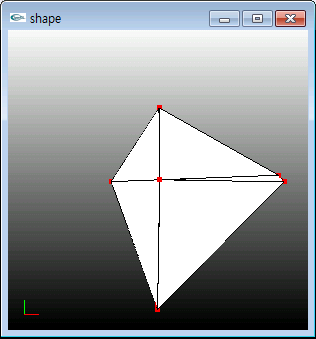
\includegraphics[width=.23\textwidth]{FIGS/Y4}
\caption{i.Y}
\end{figure}
\clearpage
\section{Know bugs/limitations}
To compute the voronoi vertex, I considered the neighboring facets of the vertex. In this process, I went through many trials and errors. I think that one \textit{function} should have only one function in a nice program. Actually, I wanted to make two function; one is for finding poles and the other is for finding antipoles. However, for computing the poles for a site, it is better to compute them in one function. Also, I had to define \textit{the maximum distance} in the process of computing them. If the distance between a site and a vertex is too large, it is difficult to view the result. For example, there is \textit{i.ellipsoid}. So, I set the \textit{MAX\_DIST} as $10000$.
\bibliographystyle{plain}
\bibliography{152cpg04}

\end{document}


